\documentclass[]{article}

\usepackage{amsfonts, amsthm, amssymb, amsmath, stmaryrd, etoolbox}
\usepackage{graphicx}
\usepackage{caption}
\usepackage{subcaption}
\usepackage{tikz}
\usetikzlibrary{matrix,arrows}
\usepackage{tikz}
\usepackage[all,2cell]{xy}
\usetikzlibrary{matrix,arrows,shapes,decorations.markings}
\definecolor{rewritecolor}{rgb}{0,.9,1}
\tikzset{rewritenode/.style={shape=circle,fill=rewritecolor,scale=0.25,font=\Huge}}
\tikzset{RWopen/.style={shape=circle,draw=black,fill=white,scale=0.5,font=\Huge}}
\tikzset{RWclosed/.style={shape=circle,fill=black,scale=0.5,font=\Huge}}
\tikzset{CDnode/.style={shape=circle,fill=white,scale=.5}}
\tikzset{zxgreen/.style={shape=circle,draw,fill=green}}
\tikzset{zxred/.style={shape=circle,draw,fill=red}}
\tikzset{zxyellow/.style={shape=rectangle,draw,fill=yellow,inner sep=2.75}}
\tikzset{zxdiamond/.style={shape=diamond,fill=black,inner sep=2.75}}
\tikzset{->-/.style={decoration={markings,mark=at position .5 with {\arrow{>}}},postaction={decorate}}}
\begin{document}


\begin{figure}
	\fbox{%
		\begin{minipage}{\textwidth}
			\centering
			%%%%%%%%%%%%%%%%%%%%%%%%%%%%%%%%%%%%%%%%
			\subcaptionbox{Spider}[\textwidth]{%
				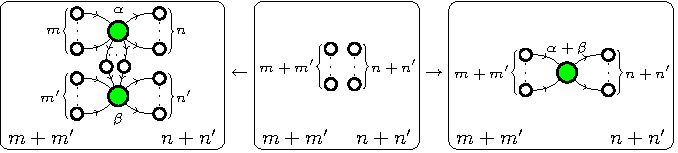
\includegraphics[scale=0.8]{2cell_spider}
			}
			\linebreak 
			\subcaptionbox{Loop}[\textwidth]{%
				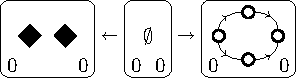
\includegraphics[scale=0.8]{2cell_loop}
			}
			\linebreak
			\subcaptionbox{Cup}[0.45\textwidth]{%
				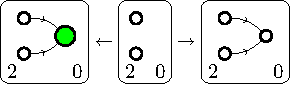
\includegraphics[scale=0.8]{2cell_cup}
			}
			\subcaptionbox{Copy}[0.45\textwidth]{%
				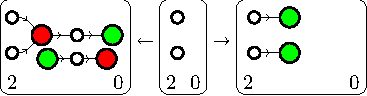
\includegraphics[scale=0.8]{2cell_copy}
			}
			\linebreak
			\subcaptionbox{Bialgebra}[\textwidth]{%
				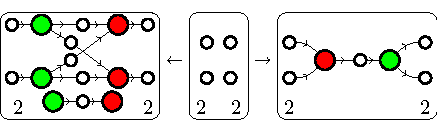
\includegraphics[scale=0.8]{2cell_bialgebra}
			}
			\linebreak
			\subcaptionbox{$\pi$-copy}[\textwidth]{%
				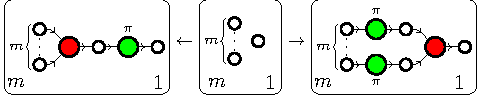
\includegraphics[scale=0.8]{2cell_pi_copy}
			}
			\linebreak
			\subcaptionbox{$\pi$-commutation}[\textwidth]{%
				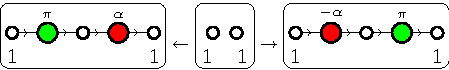
\includegraphics[scale=0.8]{2cell_pi_commutation}
			}
			\linebreak
			\subcaptionbox{Color change}[\textwidth]{%
				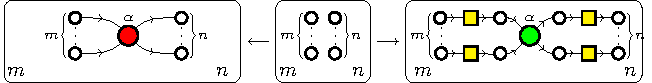
\includegraphics[scale=0.8]{2cell_color_change}
			}
			\linebreak
			\subcaptionbox{Euler decomposition}[\textwidth]{%
				\includegraphics[scale=0.8]{2cell_euler_decomposition}
			}
			\linebreak
			\subcaptionbox{diamond}[0.45\textwidth]{%
				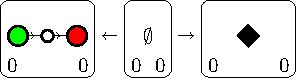
\includegraphics[scale=0.8]{2cell_diamond}
			}
			\subcaptionbox{Zero scalar}[0.45\textwidth]{%
				\includegraphics[scale=0.8]{2cell_zero_scalar}
			}
			\linebreak
			\subcaptionbox{Zero}[\textwidth]{%
				\includegraphics[scale=0.8]{2cell_zero}
			}
			\linebreak
			%%%%%%%%%%%%%%%%%%%%%%%%%%%%%%%%%%%%%%%%
		\end{minipage}
	}
	\caption{Generating $2$-cells}
	\label{fig:ZX 2cells generators}
\end{figure}




\end{document}
